\scanpage{21}
Pour tout $X\in\mathcal V$, les $A'(X)\subset A(X)$, \inserted{avec $1_{A(X)}\in A'(X)$, stable par \unsure{``signe''}} conditions équiv.

$1^\circ)$ Les $A'(X)$ stables par images inverses, images directes pour \textcircled{tout} morphisme de $\mathcal V$, et par produits [ou encore, par produits $\boxtimes$].

$2^\circ)$ \deleted{Si} a) $u\in A'(X\times Y)$, $x\in A'(X)$, alors $u_*(x)\in A'(Y)$.

b) Si $x\in A'(X)$, $y\in A'(Y)$, alors $x\boxtimes y\in A'(X\times Y)$.

c) Pour \textcircled{tout} morphisme $X-Y$ [il suffit de prendre les\hspace{1cm}] le graphe $\gamma_f=\Gamma_{f*}(1)\in A(X\times Y)$ est dans $A'(X\times Y)$.
\margin{\figure{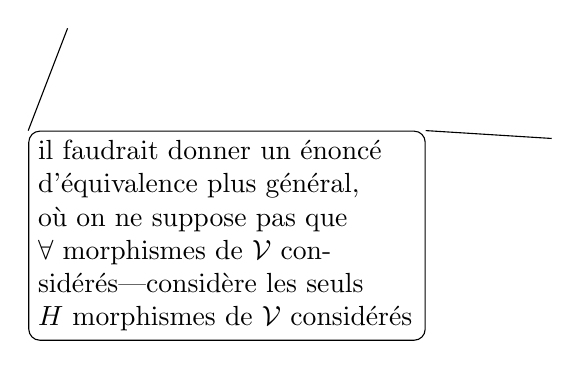
\begin{tikzpicture}\node[draw,rounded corners,text width=4.8cm] (m) {il faudrait donner un énoncé d'équivalence plus général, où on \unsure{ne suppose pas que $\uline{\forall}$ morphismes de $\mathcal V$ considérés|considère les seuls $H$ morphismes de $\mathcal V$ considérés}};\draw (m.north west)--++(.5,1.3);\draw (m.north east)--++(1.6,-.1);\end{tikzpicture}}}

\deleted{\uline{NB} Ces $A'$ correspondent aux ss-catégories (\unsure{pas pleines}) de $\mathcal V^A$ ayant \unsure{mêmes objets} que $\mathcal V^A$,}
\margin{\uline{NB} Si $\mathcal V$ a un objet final, les $A'$ correspondent exactement aux ss-catégories de $\unsure{\mathcal V_A|\mathcal V^A}$ qui ont \unsure{même ens.|ts ces} \deleted{\unsure{anneaux, et}} d'objets que $A$, stables par $\boxtimes$ de flèches, et contenant les \deleted{\unsure{projections des produits}} morphismes de $\mathcal V$ et leurs ${}^s\Gamma_f$ (il suffit ${}^s\unsure{\delta_X|\gamma_X}$).}

\uline{Dém} $1^\circ)\Longrightarrow2^\circ)$

$1^\circ$ forme \unsure{croisée} [avec $\boxtimes$] implique forme \unsure{non croisée}, car
\[
x\odot y=\delta^*(x\boxtimes y)\qquad[x,y\in A(X),\quad\delta=\operatorname{diag}_X:X-X\times X]
\]
\margin{image inverse par $\delta$}

$1^\circ$ forme \unsure{non croisée} implique forme \unsure{croisée}, car
\[
x\boxtimes y=p_1^*(x)p_2^*(y).
\]
\margin{$\boxed{\text{image inverse par }\unsure{p_i|\operatorname{pr}}}$}

a) car
\[
u_*(x)=p_{2*}(u p_1^*(x)).
\]
\margin{[De même pour $u^*(y)\in A'(X)$ si $y\in A'(Y)$]}
\margin{$\boxed{\text{image directe, inverse par }\unsure{p_i|\operatorname{pr}}}$}

b) clair

c) clair, car $1_X\in A'(X)$ par hyp.
\margin{$\boxed{\text{image directe de 1 par un graphe}}$}
\margin{$+\ \textcircled{\unsure{produit}}$}

$2^\circ)\Longrightarrow1^\circ)$. Stabilité par image \deleted{\unsure{directe}} directe: car $f_*(x)=\deleted{\unsure{\xi_f}}\gamma_f(x)$, on applique a) et c).

Stabilité par image \deleted{directe} \inserted{inverse}: car $f^*(y)=({}^{\unsure{s|t}}\gamma_f)_*(y)$, et comme $\gamma_f\in A'(X\times Y)$, on a ${}^{\unsure{s|t}}\gamma_f\in A'(Y\times X)$ (stabilité par isom),

Stabilité par $\boxtimes$ claire.
\mspage{20}
